\documentclass[14pt, a4paper]{article}

\usepackage{amssymb}
\usepackage{extsizes}
\usepackage{graphicx}
\usepackage{xcolor}
\usepackage{caption}
\usepackage{listings}
\usepackage{tabularx}
\usepackage{indentfirst}
\usepackage[T2A]{fontenc}
\usepackage[utf8]{inputenc}
\usepackage[english,russian]{babel}
\usepackage[left=30mm, right=10mm, top=20mm, bottom=20mm]{geometry}
\usepackage{ucs}

\graphicspath{{images/}}

\linespread{1.3}
\setcounter{tocdepth}{4}
\setlength{\parskip}{1.5pt}

\begin{document}	
	
	\section*{История операционных систем}
	
	{\bf Компьютер} - это программно управляемое устройство,
	которая часть времени управляется ОС, часть - приложениями.
	
	Нельзя забывать о том, что параллельно изменяется архитектура ЭВМ,
	изменяется ПО, изменются трансляторы, компиляторы, и языки программирования. Меняется все
	
	\subsection*{Этапы (поколения) ЭВМ по элементной базе}
	
	В XIX веке Ч. Бэббидж вывел идею программного управления процессами вычисления.
	Он пытался создать машину, в процессе работы поставил себе задачу разработки универсальной
	ВМ, но эта машина асболютно механическая на различных шестеренках должна была работать
	в 10сс. По его задумке управление вычислительными процессами должна управляться перфокартами,
	которые имели отверстия и, проходя через щупальца, взаимодействовали с механикой. Таким образом,
	решалась задача автоматической реализации процесса вычисления.
	
	Ада Лавлейс считается первым программистом. Ей приписывается написание первой программы, осуществляющей
	вычисление чисел Бернулли.
	
	Англичане воплотили в жизнь машину Бэббиджа.
	
	Наступают 40-е годы, и появляется идея доставки снаряда на удаленое расстояние (баллистические ракеты).
	Отсюда основная задача - ускорение вычислений.
	
	В Америке существовала т.н. баллистическая лаборатория, которая составляла таблицу траекторий.
	В 1943г. был представлен проект баллистической лаборатории под названием
	"электронный дифференциальный анализатор", которая могла вычислить траекторию за 5 минут.
	В результате появилась ВМ ENIAC (Electronic Numerical Integrator And {\underline {Computer}).
	
	До ENIAC разрабатывался компьютер на основе электромагнитных реле Mark-1 (ENIAC был на электронных лампах).
	Это одна из первых ВМ, задание операций которых выполнялась с помощью так называемых коммутационных панелей.
	Для ввода/вывода использовалась перфолента (перфокарты появились где-то в 50-х). Был добавлен АЦПУ (алфавитно-цифровое печатающее устройство (или арифметическое, надо бы уточнить))
	
	В 1945 году Фон Нейман опубликовал доклад, в котором определил основные компоненты и принципы работы ЭВМ.
	
	\begin{enumerate}
		
		\item "Универсальная ВМ должна содержать несколько основных
		устройств, а именно: арифметики,
		памяти, управления, связи с оператором";
		
		\item "Мы хотим, чтобы после начала вычислений работа ВМ не зависела от операторов";
		
		\item "Необходимо, чтобы машина могла запоминать некоторым образом, 
		не только цифровую информацию ..., но также и команды, управляющие программой, 
		с помощью которой должны производиться эти вычисления"
		
		\item "Если числа или команды представить в виде кода, и если
		эта машина может отличить число от команды, то память можно
		использовать для хранения как чисел, так и команд"
		
		\item "Помимо памяти для команд должны быть устройства, способные
		автоматически выполнять команды, которые хранятся в памяти.
		Будем называть это устройство управляющим"
		
		\item "Поскольку наша машина называется вычислительной, в ней должен быть арифметический орган"
		
		\item "Наконец, должно существовать устройство ввода-вывода,
		с помощью которого осуществляется связь между опера"
		
		\item Машина должна работать с двоичными числами, выполнять операции одну за другой, быть электронной
	
	\end{enumerate}
	
	<что-то про ЦП, просмотреть>
	
	Эти машины на реле и на пр. не имели никакой операционной системы.
	
	Поскольку команды располагаются в памяти последовательно, в процессор добавляется счетчик команд.
	Следовательно, команда не должна иметь указатель на следующую команду, адрес следующей команды вычисляется.
	
	\subsection*{Второе поколение}
	
	Начало второго поколения машин относят к началу 50-х годов, так как появилась другая элементная база
	на основе проводников - диоды и триоды. Параллельно развивались внешние устройства (не так быстро, правда).
	Уже для первых машин были созданы математические библиотеки. Первые программы писались в машинных кодах
	в абсолютных адресах (то есть отсутствовали идентификаторы данных, следовательно, нужно было знать адреса данных).
	
	Первый язык - Ассемблер (по сути, ассемблер - это мнемоническое обозначение машинных команд).
	Очень быстро появились языки высокого уровня. Машины стали менее громоздкими, более производительными,
	пожирали меньше энергии, стали более надежными.
	
	{\bf Момент:} Серийное производство ЭВМ обуславливается наличием документации.
	
	IBM разработала машину IBM 1401 - серийную ЭВМ. У ЭВМ был оператор, загружающий в машину перфокарты, компил. их -> Fortran и пр.
	
	Mainframe - отдельно стоящая машина.
	
	Встала задача эффективного использования этой машины. В результате фирма IBM предложила следующий
	вариант работы с машиной: появилась ВМ IBM 7094, а IBM 1401 стала использоваться для подготовительных действиях:
	
	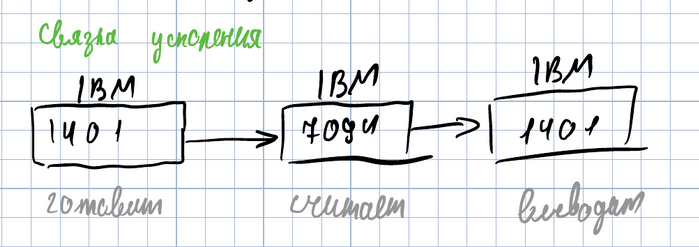
\includegraphics[width=\linewidth]{ibm7094}
	
	ОЗУ этой машины позволяло загружать множество программ,
	поэтому их можно было переключать, что позволило повысить производительность машины.
	
	Ответственность за это возлагается на {\bf операционную систему}, которая заменяла оператора.
	
	{\bf Язык управления задачами} - язык (?) переключения между задачами
	
	Формируется {\bf пакет} на перфокарте:
	
	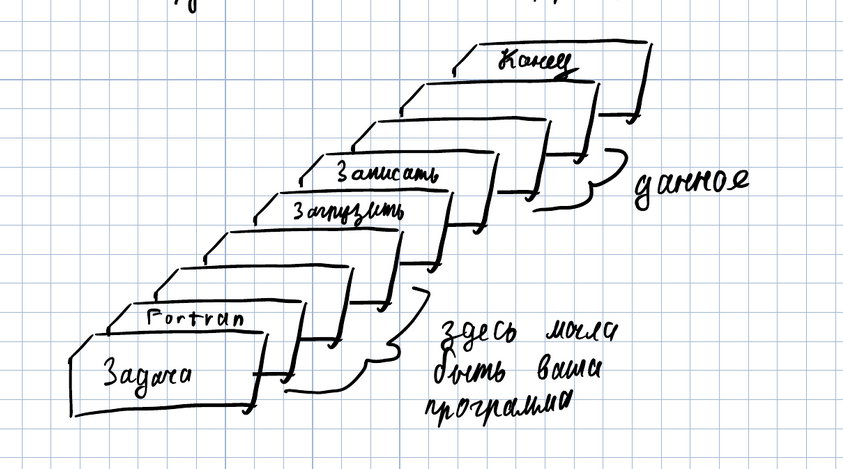
\includegraphics[width=\linewidth]{package}
	
	\subsection*{Третье поколение}
	
	В 60-е годы появляются {\bf интегральные микросхемы} и архитектура ЭВМ - новые решения организации ЭВМ (при этом принципы никуда не уходят).
	
	В IBM360 реализуется принцип распараллеливания функций - идея о том, что управление внешними устройствами
	берет на себя специальный процессор - {\bf канал}. Появляется канальная архитектура. Это привело к появлению полноценной
	системы прерываний.
	
	Получается, что процессор один, а процессов много. Как раздать всем ресурсы? Где найти все на это место? Решение - {\bf виртуальная память}
	
	В 1964 году компания MIT (Massachussets Technical University) разработала ОС CTSS (Compatible Time-Sharing System) (Совеместимая система разделения времени).
	
	На чем базируется:
	
	\begin{itemize}
		\item интегральные схемы
		
		\item большие вычислительные мощности
		
		\item потребность распараллеливания
		
		\item программирование в пакетах
		
		\item программист не связан с программой (хотим интерактивность)
		
		\item отсутствие динамического вывода информации (АЦПУ)
	\end{itemize}

	Понадобились средства динамического вывода информации -> {\bf запоминающие ЭЛТ}
	
	{\bf Терминал} - совокупность монитора и клавиатуры.
	
	Как стало возможным динамическое взаимодействие? Потребовалось изменение ОС:
	
	\begin{itemize}
		\item Пользователь не может ждать неопределенно долго. Более 3 секунд - гарантированное время ответа;
		
		\item Появляется квантование процессорного времени;
	\end{itemize}

	IBM 370 содержала virtual machine, то есть могла одновременно выполнять ОС раличного типа (времени, пакетов, ...)
	
\end{document}
